\documentclass[tikz,dvipdfmx,dvipsnames]{standalone}

\usepackage{amsmath, amssymb, amsthm, mathrsfs, amsfonts, dsfont}
\usepackage{bbm}
\usepackage{bm}
\usepackage{physics}
\usepackage{ifthen}
\usepackage{setspace}
\usepackage{mathtools}

\newcommand{\defeq}{\coloneqq}

\newcommand{\red}[1]{\textcolor{red}{#1}}
\newcommand{\blue}[1]{\textcolor{blue}{#1}}
\newcommand{\cyan}[1]{\textcolor{cyan}{#1}}
\newcommand{\gray}[1]{\textcolor{gray}{#1}}
\newcommand{\green}[1]{\textcolor{green}{#1}}
\newcommand{\brown}[1]{\textcolor{brown}{#1}}
\newcommand{\black}[1]{\textcolor{black}{#1}}
\newcommand{\orange}[1]{\textcolor{orange}{#1}}
\newcommand{\purple}[1]{\textcolor{purple}{#1}}
\newcommand{\yellow}[1]{\textcolor{yellow}{#1}}
\newcommand{\Magenta}[1]{\textcolor{Magenta}{#1}}
\newcommand{\RoyalBlue}[1]{\textcolor{RoyalBlue}{#1}}
\newcommand{\RubineRed}[1]{\textcolor{RubineRed}{#1}}
\newcommand{\ForestGreen}[1]{\textcolor{ForestGreen}{#1}}
\newcommand{\YellowOrange}[1]{\textcolor{YellowOrange}{#1}}
\newcommand{\WildStrawberry}[1]{\textcolor{WildStrawberry}{#1}}

\usetikzlibrary{calc,matrix,math}
\usetikzlibrary{decorations.pathreplacing,calligraphy}

\definecolor{c0}{HTML}{19D5A9}
\definecolor{c1}{HTML}{64FF10}
\definecolor{c2}{HTML}{FF5785}
\definecolor{c3}{HTML}{FF64DF}

\newcommand{\mono}[1]{\makebox[0.37cm][c]{#1}}

\begin{document}

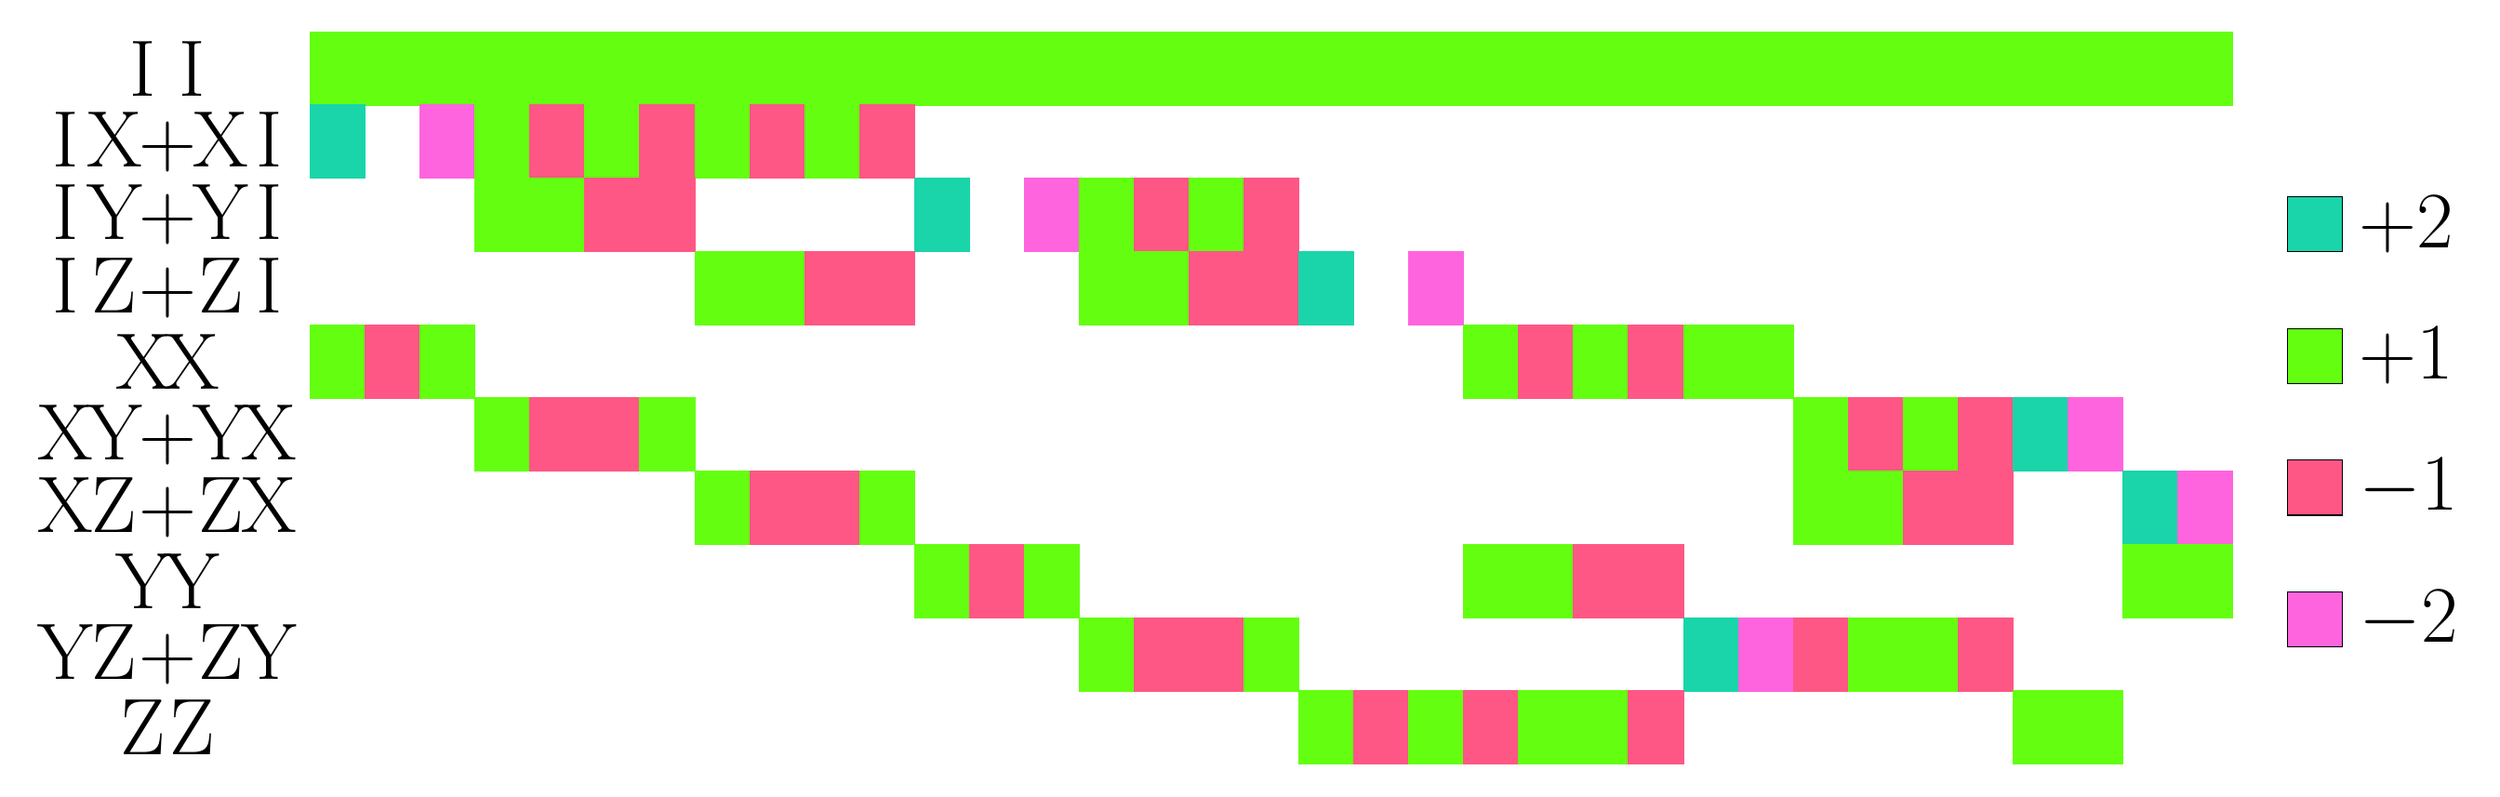
\begin{tikzpicture}[xscale=0.75]
    \foreach \color/\col/\row in {
            c1/0/0,
            c1/1/0,
            c1/2/0,
            c1/3/0,
            c1/4/0,
            c1/5/0,
            c1/6/0,
            c1/7/0,
            c1/8/0,
            c1/9/0,
            c1/10/0,
            c1/11/0,
            c1/12/0,
            c1/13/0,
            c1/14/0,
            c1/15/0,
            c1/16/0,
            c1/17/0,
            c1/18/0,
            c1/19/0,
            c1/20/0,
            c1/21/0,
            c1/22/0,
            c1/23/0,
            c1/24/0,
            c1/25/0,
            c1/26/0,
            c1/27/0,
            c1/28/0,
            c1/29/0,
            c1/30/0,
            c1/31/0,
            c1/32/0,
            c1/33/0,
            c1/34/0,
            c0/0/-1,
            c3/2/-1,
            c1/3/-1,
            c2/4/-1,
            c1/5/-1,
            c2/6/-1,
            c1/7/-1,
            c2/8/-1,
            c1/9/-1,
            c2/10/-1,
            c1/3/-2,
            c1/4/-2,
            c2/5/-2,
            c2/6/-2,
            c0/11/-2,
            c3/13/-2,
            c1/14/-2,
            c2/15/-2,
            c1/16/-2,
            c2/17/-2,
            c1/7/-3,
            c1/8/-3,
            c2/9/-3,
            c2/10/-3,
            c1/14/-3,
            c1/15/-3,
            c2/16/-3,
            c2/17/-3,
            c0/18/-3,
            c3/20/-3,
            c1/0/-4,
            c2/1/-4,
            c1/2/-4,
            c1/21/-4,
            c2/22/-4,
            c1/23/-4,
            c2/24/-4,
            c1/25/-4,
            c1/26/-4,
            c1/3/-5,
            c2/4/-5,
            c2/5/-5,
            c1/6/-5,
            c1/27/-5,
            c2/28/-5,
            c1/29/-5,
            c2/30/-5,
            c0/31/-5,
            c3/32/-5,
            c1/7/-6,
            c2/8/-6,
            c2/9/-6,
            c1/10/-6,
            c1/27/-6,
            c1/28/-6,
            c2/29/-6,
            c2/30/-6,
            c0/33/-6,
            c3/34/-6,
            c1/11/-7,
            c2/12/-7,
            c1/13/-7,
            c1/21/-7,
            c1/22/-7,
            c2/23/-7,
            c2/24/-7,
            c1/33/-7,
            c1/34/-7,
            c1/14/-8,
            c2/15/-8,
            c2/16/-8,
            c1/17/-8,
            c0/25/-8,
            c3/26/-8,
            c2/27/-8,
            c1/28/-8,
            c1/29/-8,
            c2/30/-8,
            c1/18/-9,
            c2/19/-9,
            c1/20/-9,
            c2/21/-9,
            c1/22/-9,
            c1/23/-9,
            c2/24/-9,
            c1/31/-9,
            c1/32/-9
        }{
            \draw[
                fill=\color,
                draw=\color
            ] (\col, \row) rectangle (\col + 1, \row - 1);
        }

    \foreach \row/\label in {
            -0.5/ \mono{I}\mono{I},
            -1.5/ \mono{I}\mono{X}+\mono{X}\mono{I},
            -2.5/ \mono{I}\mono{Y}+\mono{Y}\mono{I},
            -3.5/ \mono{I}\mono{Z}+\mono{Z}\mono{I},
            -4.5/ \mono{X}\mono{X},
            -5.5/ \mono{X}\mono{Y}+\mono{Y}\mono{X},
            -6.5/ \mono{X}\mono{Z}+\mono{Z}\mono{X},
            -7.5/ \mono{Y}\mono{Y},
            -8.5/ \mono{Y}\mono{Z}+\mono{Z}\mono{Y},
            -9.5/ \mono{Z}\mono{Z}
        }{
            \node[anchor=center,font=\LARGE,scale=1.8]
            at (-2.6, \row) {\label};
        }

    \begin{scope}[yscale=0.75,xshift=36cm]
        \draw[fill=c0] (0, +3.0-1.2*5) rectangle (1,    +3.0-1.2*5-1);
        \draw[fill=c1] (0, +3.0-1.2*7) rectangle (1,    +3.0-1.2*7-1);
        \draw[fill=c2] (0, +3.0-1.2*9) rectangle (1,    +3.0-1.2*9-1);
        \draw[fill=c3] (0, +3.0-1.2*11) rectangle (1,   +3.0-1.2*11-1);
        \node[anchor=west,font=\LARGE,scale=1.8] at (1, +3.0-1.2*5-0.5) {$+2$};
        \node[anchor=west,font=\LARGE,scale=1.8] at (1, +3.0-1.2*7-0.5) {$+1$};
        \node[anchor=west,font=\LARGE,scale=1.8] at (1, +3.0-1.2*9-0.5) {$-1$};
        \node[anchor=west,font=\LARGE,scale=1.8] at (1, +3.0-1.2*11-0.5) {$-2$};
    \end{scope}
\end{tikzpicture}

\end{document}